\documentclass{article}
\usepackage{xcolor}
\usepackage[final]{corl_2026}

\usepackage{amsmath,amssymb,amsthm}
\usepackage{booktabs}
\usepackage{graphicx}
\usepackage{microtype}
\usepackage{hyperref}
\usepackage{multirow}
\usepackage{subcaption}
\usepackage{tikz}
\usetikzlibrary{arrows.meta,positioning,shapes.geometric,fit,backgrounds}
\raggedbottom

\newcommand{\token}[1]{\textsc{#1}}
\newcommand{\method}{\textsc{RegretBoot}}
\newcommand{\regret}[1]{\texttt{#1}}

\title{Recoverable-Regret Bootstrapping\\for Tokenized Autonomous Driving}

\author{
  Alba Maria Tellez Fernandez\\
  \texttt{amtellezfernandez@gmail.com}\\
  Independent research prototype
}

\begin{document}

\maketitle

\begin{abstract}
Candidate-based autonomous-driving planners fail for different reasons that are often
collapsed into one aggregate score. Sometimes no generated candidate is safe. Sometimes a
safe candidate exists but the planner selects an unsafe top-1 action. Sometimes the top-1
action is safe but leaves substantial progress or imitation value on the table. We call
these three cases a generation gap, recoverable safety regret, and recoverable utility
regret. This paper introduces \method, a model-agnostic audit and bootstrapping pipeline
that turns those distinctions into training targets for candidate generators. The method
scores every candidate under public log-replay geometry, decomposes each scene by
oracle@K versus top-1 value, trains first on safety-recovery teachers, then on
utility-recovery teachers, and emits candidate-expansion requests when no in-bank safe
teacher exists. On 1,000 interaction-aware public nuPlan scenes with nine ManeuverToken
candidates per scene, the initial generator has 281 generation gaps, 346 recoverable
safety regrets, 44 recoverable utility regrets, and a 0.627 top-1 replay-failure rate.
After one bootstrapped pass, recoverable safety regret falls from 346 to 13 and top-1
failure falls from 0.627 to 0.294, while the generation gap remains fixed at 281 and
utility regret rises to 228. This is the central finding: bootstrapping can close the
selection/safety branch, but it cannot solve scenes whose candidate bank contains no safe
trajectory; once safety is recovered, a separate utility-recovery branch becomes visible.
The current evidence is deliberately bounded: it is public nuPlan log replay with a
ManeuverToken surrogate generator, not proof of closed-loop VLA safety. The contribution
is the recoverable-regret training loop and the empirical decomposition it exposes.
\end{abstract}

\keywords{autonomous driving, candidate generation, imitation learning, nuPlan,
ManeuverToken, replay safety, recoverable regret, bootstrapping}

% =====================================================================
\section{Introduction}
% =====================================================================

Modern autonomous-driving policies increasingly generate multiple possible futures, score
them, and execute one candidate. This candidate interface appears in hand-designed token
planners, imitation-learned trajectory heads, and vision-language-action (VLA) planners.
It creates an important diagnostic opportunity: when the executed action fails, we can ask
whether the planner failed to \emph{generate} a good action or merely failed to
\emph{select} one. Standard aggregate metrics hide that distinction.

This paper argues that the useful unit of analysis is recoverable regret. Given a scene
$s$, a candidate set $\mathcal{C}(s)=\{\tau_i\}_{i=1}^K$, and the planner's top-1
candidate $\tau_1$, we compare top-1 to an oracle over the same candidate bank. If
oracle@K also fails, the generator has a candidate-generation gap. If oracle@K is safe
but top-1 fails, the failure is recoverable safety regret: the candidate bank already
contained a safer trajectory. If both are safe but oracle@K has higher value, the failure
is recoverable utility regret: the planner can preserve more progress or expert
similarity without changing the generator class. These cases require different fixes, so
they should not be optimized with one undifferentiated reranking loss.

\method{} uses this decomposition as a bootstrapping loop. It does not merely rerank a
fixed bank at inference. It produces stage-specific supervision for the next generator
iteration: safety-recovery targets where the generator already proposed a safe
alternative, utility-recovery targets once safety regret is mostly removed, and
candidate-expansion requests when no safe in-bank teacher exists. The intended VLA use
case is direct: a VLA planner proposes $K$ trajectory candidates, the replay-value teacher
selects high-value in-bank targets, and the generator is distilled toward those targets.
The present paper validates the loop on a controlled ManeuverToken surrogate before
claiming a large VLA improvement.

\begin{figure}[t]
\centering
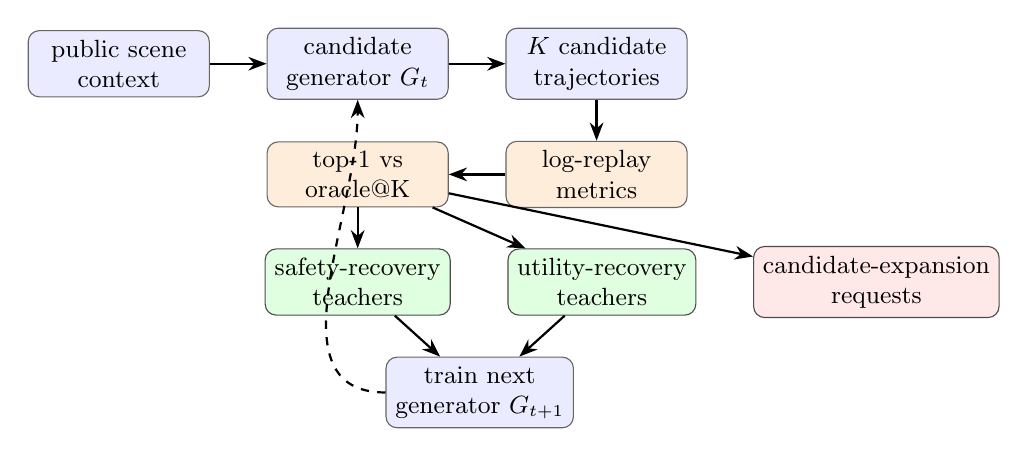
\begin{tikzpicture}[
  node distance=0.52cm and 0.72cm,
  box/.style={rectangle,rounded corners=4pt,draw=black!60,fill=blue!8,
              minimum width=2.3cm,minimum height=0.78cm,font=\small,align=center},
  val/.style={rectangle,rounded corners=4pt,draw=black!60,fill=orange!14,
              minimum width=2.3cm,minimum height=0.78cm,font=\small,align=center},
  targetbox/.style={rectangle,rounded corners=4pt,draw=black!70,fill=green!12,
              minimum width=2.35cm,minimum height=0.78cm,font=\small,align=center},
  warn/.style={rectangle,rounded corners=4pt,draw=black!70,fill=red!9,
              minimum width=2.35cm,minimum height=0.78cm,font=\small,align=center},
  arr/.style={-Stealth,thick}
]
  \node[box] (scene) {public scene\\context};
  \node[box,right=of scene] (gen) {candidate\\generator $G_t$};
  \node[box,right=of gen] (bank) {$K$ candidate\\trajectories};
  \node[val,below=of bank] (eval) {log-replay\\metrics};
  \node[val,left=of eval] (oracle) {top-1 vs\\oracle@K};
  \node[targetbox,below=of oracle] (safe) {safety-recovery\\teachers};
  \node[targetbox,right=of safe] (util) {utility-recovery\\teachers};
  \node[warn,right=of util] (expand) {candidate-expansion\\requests};
  \node[box,below=of safe,xshift=1.55cm] (next) {train next\\generator $G_{t+1}$};

  \draw[arr] (scene) -- (gen);
  \draw[arr] (gen) -- (bank);
  \draw[arr] (bank) -- (eval);
  \draw[arr] (eval) -- (oracle);
  \draw[arr] (oracle) -- (safe);
  \draw[arr] (oracle) -- (util);
  \draw[arr] (oracle) -- (expand);
  \draw[arr] (safe) -- (next);
  \draw[arr] (util) -- (next);
  \draw[arr,dashed] (next.west) to[out=180,in=270] (gen.south);
\end{tikzpicture}
\caption{\method{} separates candidate-generation failure from recoverable selection
regret. Safety and utility cases produce in-bank teacher trajectories for bootstrapping.
Generation-gap cases do not: they request a richer candidate distribution.}
\label{fig:loop}
\end{figure}

The empirical result is intentionally narrow and reproducible. We use public nuPlan
scenes~\citep{caesar2021nuplan}, an interaction-aware sampler, and logged future actors
to evaluate the replay clearance of every token. The current generator is a
ManeuverToken bank of nine canonical responses. This surrogate is useful because every
candidate can be scored exactly and the top-1 choice can be changed without confounding
the candidate set. The same JSON/JSONL candidate interface also accepts external VLA
outputs, but VLA dumps are used for regret claims only after every candidate has replay
and utility metrics attached.

We make four contributions.

\begin{enumerate}
  \item \textbf{Recoverable-regret decomposition.} We define generation gap,
    recoverable safety regret, and recoverable utility regret for candidate driving
    planners using top-1 versus oracle@K under the same candidate bank.

  \item \textbf{Bootstrapped candidate curriculum.} We turn the decomposition into a
    generator-training curriculum: safety recovery first, utility recovery second, and
    candidate expansion for scenes with no safe in-bank teacher.

  \item \textbf{Public interaction replay audit.} On 1,000 public nuPlan interaction
    scenes, the initial token generator exposes all three regimes at scale: 281
    generation gaps, 346 recoverable safety regrets, and 44 utility regrets.

  \item \textbf{One-step lifecycle evidence.} A bootstrapped generator pass reduces
    recoverable safety regret from 346 to 13 and top-1 replay failure from 0.627 to
    0.294, while leaving the generation gap unchanged. This validates the split: in-bank
    safety regret is learnable; missing safe candidates require generator expansion.
\end{enumerate}

% =====================================================================
\section{Related Work}
% =====================================================================

\paragraph{Imitation learning and long-tail driving.}
Behavior cloning suffers from covariate shift~\citep{pomerleau1989alvinn,ross2011dagger},
and driving systems often degrade on rare interaction compositions even when common-case
performance is strong~\citep{bansal2018chauffeurnet,hu2023planning}. Larger sensor-fusion
and VLA models improve representation and scale~\citep{chitta2022transfuser,brohan2023rt2},
but they do not by themselves answer whether a failure is due to missing candidates or bad
selection among candidates.

\paragraph{Candidate planners and VLA grounding.}
Latent VLA driving systems such as LaST-VLA~\citep{luo2026lastvla} argue that planning
should be grounded in geometry and dynamics rather than only textual reasoning. Our work
is complementary: it instruments the action-candidate interface that such systems must
ultimately use. A grounded generator can still fail if its top-1 candidate is not the best
candidate it generated. Conversely, no reranker can recover a scene where oracle@K is
unsafe. The paper's core distinction is therefore between generation gap and recoverable
selection regret.

\paragraph{Reranking, self-training, and bootstrapping.}
Candidate reranking is a known way to improve top-1 decisions. \method{} is not presented
as a novel scoring head alone. Its contribution is to use replay-measured regret to decide
which examples should train the next generator iteration and which examples require
candidate expansion. The safety-recovery and utility-recovery phases produce teacher
trajectories; generation-gap scenes do not. This prevents the method from treating all
planner failures as more labels for the same selector.

% =====================================================================
\section{Method}
\label{sec:method}
% =====================================================================

\subsection{Candidate Interface}
\label{sec:method:candidates}

For each scene $s$, a planner or generator $G_t$ emits a finite candidate bank
\[
  \mathcal{C}_t(s)=\{\tau_1,\ldots,\tau_K\},
\]
where each $\tau_i$ is a trajectory candidate with an identifier, optional token label,
and per-candidate metrics. The current nuPlan surrogate uses the nine ManeuverTokens in
Table~\ref{tab:tokens}; the same file format accepts sampled or beam-search trajectories
from a VLA generator.

\begin{table}[t]
\centering
\caption{ManeuverToken candidate bank used for the public surrogate experiment. The method
does not depend on these hand-written tokens; it only requires a candidate bank with
attached replay and utility metrics.}
\label{tab:tokens}
\footnotesize
\begin{tabular}{lccl}
\toprule
Token & Speed scale & Lateral offset & Role \\
\midrule
\token{stop}           & 0.00 & 0.0  & hard stop \\
\token{crawl}          & 0.15 & 0.0  & cautious forward \\
\token{maintain}       & 1.00 & 0.0  & nominal progress \\
\token{slow\_yield}    & 0.50 & 0.0  & yielding progress \\
\token{nudge\_left}    & 0.80 & +0.9 & mild left avoidance \\
\token{nudge\_right}   & 0.80 & -0.9 & mild right avoidance \\
\token{evasive\_left}  & 0.70 & +2.2 & strong left avoidance \\
\token{evasive\_right} & 0.70 & -2.2 & strong right avoidance \\
\token{lane\_recover}  & 0.90 & 0.0  & lane-center recovery \\
\bottomrule
\end{tabular}
\end{table}

Each candidate is evaluated against logged future actors. A candidate is replay-failed if
its minimum replay clearance falls below the near-miss threshold. This is a conservative
future-geometry test, not a reactive closed-loop simulator: logged actors do not respond
to the ego candidate.

\subsection{Replay Value}
\label{sec:method:value}

We assign each candidate a replay value
\begin{equation}
  V(s,\tau) =
  -\lambda_f \mathbf{1}[\tau\ \text{replay-fails}]
  + w_p\,p(s,\tau)
  - w_a\,\mathrm{ADE}_{3s}(s,\tau)
  - w_f\,\mathrm{FDE}_{3s}(s,\tau)
  + w_c\,c(s,\tau),
  \label{eq:value}
\end{equation}
where $p$ is route progress, $\mathrm{ADE}_{3s}$ and $\mathrm{FDE}_{3s}$ compare the
candidate to logged ego motion, and $c$ is optional clearance reward. The main reported
artifacts use $\lambda_f=250$, $w_p=1$, $w_a=2$, $w_f=0$, and $w_c=0$. These weights are
not claimed to be universal; they define the replay teacher used for the current audit.

Let
\[
  \tau^\star(s)=\arg\max_{\tau\in\mathcal{C}_t(s)} V(s,\tau)
\]
be oracle@K inside the generated bank, and let $\tau_1(s)$ be the generator's selected
top-1 candidate. The recoverable regret is
\begin{equation}
  R(s)=\max(0, V(s,\tau^\star)-V(s,\tau_1)).
\end{equation}

\subsection{Regret Taxonomy}
\label{sec:method:taxonomy}

Each valid scene is assigned one of four outcomes:

\begin{description}
  \item[Generation gap.] Oracle@K replay-fails. No candidate in the bank is safe under the
    replay metric, so there is no in-bank teacher trajectory.
  \item[Recoverable safety regret.] Oracle@K is replay-safe but top-1 replay-fails. The
    candidate bank contains a safe teacher that the generator failed to select.
  \item[Recoverable utility regret.] Oracle@K and top-1 are both replay-safe, but
    $V(s,\tau^\star)-V(s,\tau_1)$ exceeds a utility threshold. The scene is safe but
    inefficient or poorly matched to logged ego motion.
  \item[Minor regret.] Top-1 is replay-safe and the value gap is below the utility
    threshold.
\end{description}

The taxonomy is deliberately ordered. Safety regret takes precedence over utility regret;
generation gap takes precedence over both because no in-bank target can repair the scene.

\subsection{Bootstrapped Curriculum}
\label{sec:method:curriculum}

\method{} converts the taxonomy into training data for the next generator iteration.
For each recoverable safety-regret scene, the target is the oracle@K candidate and the
loss weight is proportional to normalized regret. After a safety-recovery pass, the
pipeline re-audits the new generator $G_1$ and extracts utility-recovery targets from the
remaining safe-but-suboptimal scenes. Generation-gap scenes are emitted as
candidate-expansion requests instead of training labels, because distilling toward an
unsafe oracle would teach the generator to imitate a failure.

This staging is the key methodological point. A single reranker can only exploit existing
candidate diversity. \method{} asks whether the generator itself improved: recoverable
safety regret should fall after safety bootstrapping; utility regret may rise because safe
but low-utility decisions become visible; generation gap should remain unchanged unless
the candidate distribution expands.

% =====================================================================
\section{Experiments}
\label{sec:experiments}
% =====================================================================

\subsection{Public Interaction Replay Setup}

We use a 1,000-scene interaction-aware public nuPlan replay subset. Scenes are sampled to
avoid the smallest/easiest databases and to prefer dynamic interactions using actor
density, minimum actor distance, closing/TTC-style risk when available, ego speed,
route/intersection context, and expert braking/steering magnitude. Each scene has nine
ManeuverToken candidates and replay metrics for all candidates, producing 9,000 scored
candidate trajectories. The validator marks the dump as analysis-ready: all 1,000 scenes
and all 9,000 candidates have replay and utility metrics attached.

\paragraph{Claim boundary.}
The reported replay metric uses logged future actor geometry. It supports claims about
future-geometry infeasibility and recoverable candidate regret. It does not prove closed-loop
controller safety, because actors do not react to ego actions. We use the closed-loop
bridge only as infrastructure in this draft, not as the main evidence claim.

\subsection{Initial Regret Decomposition}
\label{sec:exp:g0}

Table~\ref{tab:lifecycle} shows the main lifecycle result. The initial generator $G_0$
has 281 generation gaps, 346 recoverable safety regrets, and 44 recoverable utility
regrets. Its top-1 replay-failure rate is 0.627, while oracle@K replay-failure rate is
0.281. The difference is the recoverable selection surface: many failures are not caused
by the absence of any safe candidate, but by selecting the wrong candidate from a bank
that already contains a safer one.

\begin{table}[t]
\centering
\caption{Recoverable-regret lifecycle on 1,000 interaction-aware public nuPlan scenes.
The bootstrapped pass closes most recoverable safety regret but does not change the
generation gap, as expected when the candidate bank size and token library remain fixed.}
\label{tab:lifecycle}
\footnotesize
\begin{tabular}{lrrrrrr}
\toprule
Stage & Gen. gap & Safety regret & Utility regret & Mean regret & Top-1 fail & Oracle fail \\
\midrule
$G_0$ & 281 & 346 & 44  & 79.649 & 0.627 & 0.281 \\
$G_1$ & 281 & 13  & 228 & 8.056  & 0.294 & 0.281 \\
\midrule
$\Delta$ & 0 & -333 & +184 & -71.594 & -0.333 & 0.000 \\
\bottomrule
\end{tabular}
\end{table}

\subsection{Bootstrapped Safety Pass}
\label{sec:exp:g1}

The $G_1$ stage is a one-pass bootstrapped surrogate: scenes with recoverable safety
regret are moved toward replay-safe in-bank teachers, then the candidate set is re-audited
under the same replay-value definition. Recoverable safety regret falls from 346 to 13,
and top-1 replay failure falls from 0.627 to 0.294. Mean regret drops from 79.649 to
8.056. The oracle failure rate remains 0.281 because the same 281 generation-gap scenes
still contain no replay-safe candidate in the bank.

This pattern is the desired sanity check for the method. If the safety bootstrap had also
reduced the generation gap, the pipeline would be silently changing the candidate set or
the metric. If it had not reduced recoverable safety regret, the teacher targets would not
be learnable. Instead, the lifecycle separates what the current generator can repair from
what requires candidate expansion.

\subsection{Curriculum Targets}
\label{sec:exp:curriculum}

Table~\ref{tab:curriculum} summarizes the emitted training curriculum. Phase 1 contains
346 safety-recovery targets with high mean regret (226.103), dominated by
\token{crawl}, \token{slow\_yield}, \token{evasive\_right}, and \token{stop} teachers.
After that safety branch is mostly closed, phase 2 contains 228 utility-recovery targets
with much smaller mean regret (5.696), dominated by \token{maintain} and
\token{nudge\_right}. Phase 3 contains 281 candidate-expansion requests: these scenes
have no safe in-bank teacher and should not be used as ordinary distillation labels.

\begin{table}[t]
\centering
\caption{Bootstrapped curriculum produced by the $G_0\rightarrow G_1$ lifecycle. Safety
and utility phases have in-bank teacher trajectories. Candidate-expansion scenes do not.}
\label{tab:curriculum}
\scriptsize
\resizebox{\linewidth}{!}{%
\begin{tabular}{lrrrp{0.54\linewidth}}
\toprule
Phase & Count & Mean regret & Mean weight & Dominant teachers or requests \\
\midrule
safety recovery & 346 & 226.103 & 2.806 &
\token{crawl}: 92, \token{slow\_yield}: 96, \token{evasive\_right}: 64,
\token{stop}: 46, \token{nudge\_right}: 28 \\
utility recovery & 228 & 5.696 & 0.767 &
\token{maintain}: 135, \token{nudge\_right}: 47, \token{evasive\_right}: 17,
\token{lane\_recover}: 15 \\
candidate expansion & 281 & n/a & n/a &
no in-bank replay-safe teacher; request new samples or richer generator support \\
\bottomrule
\end{tabular}
}
\end{table}

\subsection{Interpretation}
\label{sec:exp:interpretation}

The result does not say that one fixed risk penalty or one reranker solves driving. It
says the lifecycle discovers two different optimization branches. The first branch is
recoverable safety: $G_0$ often generated a safe candidate but did not choose it, and
bootstrapping largely fixes that branch. The second branch is utility recovery: once the
top-1 candidate is usually safe, many scenes still have a better in-bank candidate by
progress and logged-ego similarity. The third branch is candidate expansion: 281 scenes
remain unsafe even under oracle@K, so no selector or calibrator can repair them without
new candidates.

This is also why the method should be evaluated by lifecycle changes rather than a single
top-1 score. A static reranker can reduce top-1 failure, but it does not answer whether
the generator's future candidate distribution improves or whether the remaining failures
are unrecoverable with the current bank. \method{} makes that accounting explicit.

% =====================================================================
\section{Discussion}
\label{sec:discussion}
% =====================================================================

\paragraph{What is new relative to reranking.}
A learned value calibrator over candidates is not enough by itself; it is close to
standard reranking. The contribution here is the training loop around the calibrator:
measure oracle@K regret, separate safety from utility from generation gap, distill only
recoverable in-bank teachers, and route oracle-failed scenes to candidate expansion.
This creates a falsifiable lifecycle prediction: safety regret should fall before utility
regret is optimized, while generation gap should not move unless the generator emits new
candidate modes.

\paragraph{Why the utility branch rises.}
The increase from 44 to 228 utility-regret scenes is not a regression under the taxonomy.
It means safety failures have been converted into safe but suboptimal decisions. The next
iteration should optimize the utility branch with a different loss scale and different
teacher distribution, rather than continuing to apply the same safety-heavy objective.

\paragraph{Relation to VLA planners.}
The candidate interface is intentionally model-agnostic. A VLA generator can be plugged in
if it emits $K$ candidate trajectories and top-1 metadata. The current repository includes
conversion and validation tools for this path, but this paper does not claim VLA top-1
improvement until replay and utility metrics are attached to every generated candidate.
The ManeuverToken experiment is therefore a controlled proof of the regret-bootstrap
mechanism, not a claim that a released VLA planner has already been improved.

% =====================================================================
\section{Limitations}
\label{sec:limitations}
% =====================================================================

\paragraph{Log replay is not closed-loop safety.}
Logged actors do not react to the ego candidate. Replay infeasibility is a public,
reproducible future-geometry signal, but it is not equivalent to closed-loop collision
under reactive traffic. The correct claim is that replay risk is a useful calibration and
bootstrapping signal for candidate planners.

\paragraph{Current generator is a surrogate.}
The reported lifecycle uses a nine-token ManeuverToken generator. This makes the
candidate bank auditable, but it also fixes the candidate distribution. The unchanged
281-scene generation gap is partly a property of that limited bank. A VLA or sampling
generator must be evaluated by whether it reduces this gap while preserving candidate
diversity.

\paragraph{The $G_1$ pass is one-step bootstrapping, not a full policy-training result.}
The current $G_1$ artifact demonstrates the accounting and safety-recovery branch. A full
generator-training paper should run multiple regeneration cycles, report diversity and
oracle@K changes, and compare static reranking against actual generator improvement.

\paragraph{Value weights define a teacher.}
Equation~\ref{eq:value} uses a safety-dominant replay value. Changing the failure penalty
or progress/ADE weights changes which utility targets are emitted. This is why the paper
reports the lifecycle and curriculum rather than presenting one weight setting as a
universal driving objective.

% =====================================================================
\section{Conclusion}
% =====================================================================

Candidate planners need more than a better top-1 scorer. They need to know whether a
failure was recoverable inside the candidate bank. \method{} provides that accounting. On
1,000 public nuPlan interaction scenes, the initial ManeuverToken generator has a large
recoverable safety branch: 346 scenes where a safe in-bank teacher exists but top-1 fails.
One bootstrapped pass reduces that branch to 13 and cuts top-1 replay failure from 0.627
to 0.294. The unchanged 281-scene generation gap shows the boundary of the method: no
selector can repair a bank that contains no safe candidate. The newly exposed
228-scene utility branch defines the next training phase.

The scientific claim is therefore not that replay safety solves closed-loop AV planning.
It is that recoverable-regret bootstrapping turns candidate-planner failures into
different training tasks: recover safety when a safe teacher exists, recover utility when
safety is already achieved, and expand the generator when oracle@K still fails. That is
the mechanism a VLA candidate generator should optimize next.

\acknowledgments{Developed independently as a research prototype using public nuPlan-style
replay artifacts and internal repository tooling.}

\bibliography{paper}

\end{document}
